\chapter{The train case} % FIXME this name sucks

Let's summarize the model.
We know $g(x,y)$ and we know that there is a $h(x,y)$ such that
\[ g(x,y) = h(x,y) * f(x,y) + e(x,y). \]
We would like to find $f(x,y)$.
To obtain it, we need to deconvolve $g(x,y)$ with a method
robust to the noise $e(x,y)$.

However, we don't know $h(x,y)$ so we first need to estimate it
in a way that is also robust to the noise.
It is easier to estimate $h(x,y)$ if we make some assumptions.
For our problem, we have a motion blur which means that
$h(x,y)$ only depends on an angle and a length which are
respectively the blur angle and the number of
pixel on which each pixel depends.

Once we have an estimate of $h(x,y)$, we deconvolve
$g(x,y)$ to get an estimate $\hat{f}(x,y)$.
For some deconvolution methods, we need an estimate of
some properties of the noise which is done only using $g(x,y)$.

\section{Estimation of the PSF}
In the spatial domain, we have
\[ g = h * f \]
so in the fourier domain
\[ G = H \cdot F. \]
Since $h$ is a window, which is like
$\frac{1}{L}
\begin{pmatrix}
  1 & 1 & \cdots & 1
\end{pmatrix}$ rotate at the angle of blur.
It's fourier transform $H$ is therefore
a 2-D $\sinc$ at the angle of blur
which can be detected in various ways.

In~\cite{krahmer2006blind},
Radon and Cepstrum methods are presented.
Radon is said to be more appropriate for angle
estimation and Cepstrum more appropriate for length
estimation while being quite competitive to Radon
for angle estimation when the length of the blur
is small.
However, \cite{oliveira2007blind} says that
\cite{krahmer2006blind} is wrong and by adapting
the way Radon is computed like he has done
in~\cite{oliveira2006implementation},
it can also be used with success for small length and
he doesn't need normalization
(we'll see in section~\ref{sec:rt} what
normalization is,
understand it now is not necessary).
We have however not found its source code of
``exact Radon transform''.

\subsection{Angle estimation with Radon}
\subsubsection{Preliminaries}
The idea is to detect the $\sinc$ shape in $H$.
The problem of $G$ is that even
after making the image 0-mean,
it's value at the center are so huge that the others
are negligeable.
We therefore compute its $\log$ or rather the $\log$
of its absolute value to avoid undefined value.
There is still problems with very small values which
have a $\log$ that can be very far in the negative axis
so we compute $S = \log(1 + |G|)$.

\begin{myfig}{cameraman_F_diff}
  {Effect of the blur on the fourier transform}
  \mysubfig{cameraman_F}{$S$ for the cameraman.}{0.32}
  \mysubfig{cameraman_F_replicate_40-30}{$S$ for the cameraman with a blur of $(40, 30)$ with ``replicate''.}{0.32}
  \mysubfig{cameraman_F_circular_40-30}{$S$ for the cameraman with a blur of $(40, 30)$ with ``circular''.}{0.32}
\end{myfig}

In the figure~\ref{fig:cameraman_F_circular_40-30},
we can see the effet of the blur on $S$.
$S$ for the original image is in the
figure~\ref{fig:cameraman_F}.
However, as mentioned in \cite{krahmer2006blind},
there is a problem at angles 0 and $\frac{\pi}{2}$ which
can be seen in the figure~\ref{fig:cameraman_F_replicate_40-30}.
The reason is that when we do a fft,
the signal is supposed to be periodic.
However, since we blur and then take a rectangular image,
the pixels at each sides of the borders are influenced
by pixels out of the image.
If those pixels are not the same of the pixels at the other side
(as if the image were periodic),
$g$ will be like a blurred image at $(L,\alpha)$ plus
some problems at the borders of a rectangle.
Since those problems appears along $x$ and $y$ axis,
that creates artifacts at $0$ and $\frac{\pi}{2}$ in $G$.

The figure~\ref{fig:cameraman_F_circular_40-30}
and~\ref{fig:cameraman_F_replicate_40-30} are excellent
examples.
When we blur an image artificially, we need to extrapolates
the pixels beyond the borders.
\begin{enumerate}
  \item[circular] We consider an infinite image make of
    the same image repetitively.
  \item[replicate] The pixel beyond the border is the
    same as the pixel at the border.
\end{enumerate}
We can see that ther is no problem with
the figure~\ref{fig:cameraman_F_circular_40-30}
since a circular image is what the fft is expecting.
fft therefore recognize exactly the periodic image
blurred by the PSF and there is no artifacts
at 0 and $\frac{\pi}{2}$.

Sadly, for a real blurred image, we cannot decide the
way it is blurred and the chance that the image is
periodic is very small.

\cite{krahmer2006blind} gives a solution for this
which is multiplying our image by a hann window before
applying the fourier transform like done
in the figure~\ref{fig:sagar-hann}.
This methods works very well but unfortunately,
we haven't seen it immediately so we have taken a lot
of time trying to find other solutions.

We have isolated the radon in
the listing~\ref{lst:angle_estimator} and
the listing~\ref{lst:robust_angle_estimator} contains
our solution which calls it with the image at different
angles.
It does the following for the different angles
(by default, it is 0 and $\frac{\pi}{4}$)
\begin{enumerate}
  \item Rotate the image at this angle.
  \item Take a square in the image.
  \item Call the listing~\ref{lst:angle_estimator} which
    returns the $\var$ for each angle between 0 and $\pi$.
  \item Sets borders to $\{0\}$, $\{\frac{\pi}{2}\}$
    and $\{\pi\}$.
  \item While the distance between the $\argmax$ and the
    closest border is less that a $\epsilon > 0$ chosen
    beforehand, we increase the border to this angle.
  \item If there is no border left, no angle is chosen.
\end{enumerate}
That way, we ignores the peeks at $0$, $\frac{\pi}{2}$
and $\pi$ along with their influence with the angles
closes to them.
We are sure to take an angle whre there is a peek
which is not one of the 3 peeks at 0, $\frac{\pi}{2}$, $\pi$.

Once we have done that for all the angles,
we take the maximum of their respective $\var$.

Since we rotate the image in spatial domain and then crop
a square, the artifacts at 0, $\frac{\pi}{2}$ and $\pi$ are
not rotated with the $\sinc$.

Sadly, the rotating removes the clarity of the blur since
we need to do interpolation to get back square pixels.
The hann window is therefore a prefered solution.

Lastly, \cite{krahmer2006blind} warns us that the angle
detected by radon will not be the same than the angle
we are looking for if the image is not squared.
Indeed, if it is not squared, the sampling frequency
will still be the same for both dimensions since
the pixel are squares but the period of periodicity
in the spatial domain will not be the same.
The samply frequency on the frequency domain will therefore
be different wich mean that ``pixels'' in the frequency
domain will not be squares.
They give a formula to make the translation.
Our approach was rather simpler.
If the image is not squared, square it by cropping the
longest dimension.

\subsubsection{The Radon transform (RT)}
\label{sec:rt}
The idea of Radon is, for a certain angle $\theta$,
integrate over the perpendicular lines of the line at
angle $\theta$ passing by $(0,0)$.
The value of each integral is a function of the
point at which the perpendicular line intersects the
line.

More precisely, de define a new frame $(x',y')$
which is $(x,y)$ rotated by $\theta$ counterclockwise.
We then define
\[ R_\theta(x') = \int_{y_0'(x')}^{y_1'(x')} f'(x',y') \dif y' \]
where $f'$ is the image in the new frame,
$y_0'(x')$ is the smallest of $y$ so that $f'(x',y_0'(x'))$ is in the image
and $y_1'(x')$ is the biggest such value.

\begin{myfig}{ones}
  {Analysis of the RT on an unit matrix (filled with ones)}
  \mysubfig{ones-Rad}{RT of an unit matrix.}{0.45}
  \mysubfig{ones-Var}{Variance and max for each angle of the RT.}{0.45}
\end{myfig}

The problem is that the perpendicular line is longer for angles
like $\frac{\pi}{4}$ at $x' = 0$.
We can see this in the figure~\ref{fig:ones-Rad},
this is a RT of an unit matrix so the value of the RT is
basically $y_1'(x') - y_0'(x')$.
At $(\ang{45},0)$, we can see that it is maximum.
What \cite{oliveira2007blind} suggests is to use a fixed
value for $y_0'$ and $y_1'$ but that's not
what the implementation of matlab does.
This is why he implements a new RT in~\cite{oliveira2006implementation}.

Since we've not found it's source code,
we'll just do a simple normalization
by dividing by the length of the line,
which is $y_1'(x') - y_0'(x')$ as
suggested by~\cite{krahmer2006blind}.
To do that easily,
we divide our RT pointwise by the
RT of an unit image.

Now that we have solved this normalization problem,
we can see the effect of the angle of the blur $\alpha$
on the normalized RT.

When $\theta = \alpha$,
$x'$ is perpendicular to the peeks of the $\sinc$ so
we integrate along the peeks of the $\sinc$.
For example, in the \figref{sagar-S}, we can see
that the peeks are at an angle of $\ang{9}$ since the
blur is at $\ang{171}$.
$R_\alpha$ can therefore be distinguished by the value
of its $\max$ or $\var$ which will be greater than the
others.
\cite{oliveira2007blind} suggests to use the $\var$
but we have found images where the $\max$ was more
accurate.
Mostly while we had not found the hann method.
With hann, the $\var$ performs almost always
better than the $\max$.

If we compute the $\var$, we must crop $(x',R_\theta(x'))$ when
this $x'$ is out of the image for some other angle.
We can see in the figure~\ref{fig:sagar-RadNorm} that
there is a lot more values at \ang{45} that for other angles.
It is therefore cropped to figure~\ref{fig:sagar-RadFocus}.

As we can see with Sagar, if we had not normalized,
the $\var$ would have gave use \ang{135}
(see figure~\ref{fig:sagar-Var}) while the $\max$
would still be correct
(see figure~\ref{fig:sagar-max}) but almost.
With a smaller blur (for Sagar, we have $L = 25$) we would
have found \ang{135} also or \ang{45}.

With the normalization, \figref{sagar-VarN} and
\figref{sagar-maxN} agrees with \ang{171} which is the right
answer.

\begin{myfig}{sagar}
  {Analysis of the normalization of radon for Sagar which is an imaged blur at
  $(25,\ang{171})$.}
  \mysubfig{sagar-hann}{Square in the image multiplied by a hann window.}{0.4}
  \mysubfig{sagar-S}{$S$ where we can clearly see the $\sinc$.}{0.4}
  \mysubfigg{sagar-Rad}{RT of $S$.}{0.2}{trim=8cm 0cm 8cm 0cm, clip, height=4cm}
  \mysubfigg{sagar-RadNorm}{Normalized RT of $S$.}{0.2}{trim=8cm 0cm 8cm 0cm, clip, height=4cm}
  \mysubfigg{sagar-RadFocus}{Normalized and cropped RT of $S$.}{0.2}{trim=7cm 0cm 7cm 0cm, clip, height=4cm}
\end{myfig}
\begin{myfig}{sagar-plot}
  {$\var$ and $\max$ of the RT of $S$ for Sagar}
  \mysubfig{sagar-Var}{$\var$ of the RT.}{0.4}
  \mysubfig{sagar-VarN}{$\var$ of the normalized RT.}{0.4}
  \mysubfig{sagar-max}{$\max$ of the RT.}{0.4}
  \mysubfig{sagar-maxN}{$\max$ of the normalized RT.}{0.4}
\end{myfig}

\subsection{Angle estimation with Gabor}
The Gabor filter is a gaussian filter modulated by a sinusoidal wave. The function of this filter is given by:
\begin{equation}
B(x,y)=dfrac{1}{2\pi \sigma_x \sigma_y} exp\left[-\frac{1}{2}\left(\frac{x^2}{\sigma_x^2}+ \frac{y^2}{\sigma_y^2} \right) -j\omega(xcos\phi + ycos\phi)\right],
\label{filtreGabor}
\end{equation}
where $\sigma_x$ and $\sigma_y$ are the standard deviations in the $x$ and $y$ directions. The parameters $\phi$ and $\omega$ are the direction and the frequency of the filter respectively. Only $\phi$ will vary while the other parameters stay fixed. According to the article (?? ref dash20.. ??), experimentation has shown that good values for $\sigma$ and $\omega$ are $3$ and $1.75$ respectively. The method consists in applying the Gabor filter to the power spectrum of the blurred image and then detecting the blur angle $\theta_{blur}$ by searching for the $\phi$ that gives the highest response value. This value can be calculated using $L_2$ norm. The $\phi$ obtained by this method is the blur angle. Here are the steps of the algorithm:

1. computation of the spectrum of the blurred image by a two dimensional Fourier transform\\
2. taking the logarithm of it\\
3. convolving this with the Gabor function given by equation $(\ref{filtreGabor})$ for different $\phi$, the result is $R(\phi)$\\
4. for every $\phi$, taking the $L_2$ norm: $||R(\phi)||$
5. the blur angle is the parameter $phi$ that gives the biggest norm:
\begin{equation}
\theta_{blur} = arg \left\lbrace max_{\phi}R(\phi)\right\rbrace.
\end{equation}

This algorithm is implemented by our matlab function $angle_estimator_Gabor(f,thetamin, thetamax)$, where the input $f$ is the blurred image. The parameter $\phi$ will vary from $thetamin$ to $thetamax$. If those inputs are not specified, we set them to $0$ for $thetamin$ and $180$ for $thetamax$.

%TODO Resultats en images

\subsection{Length with Cepstrum}
We can verify that in
\[ \log(\F(|\log(|g|)|)), \]
along the angle of blur,
there is a peek at the center and a second peek
at a distance of $L$ in units of the discretization.

A peek detection algorithm can then be applied
to find $L$.

The problem is that it depends on the angle
and is sensible to errors in the angle
estimation.

\section{Deconvolution}
\subsection{Inverse filter}
The first and most obvious type of deconvolution is using an inverse filter. We have a blurred image $g$, we found an estimation of the psf ($h_e$) in the previous section %TODO ça sera tjs des sections ?
. So we are theoretically ready to find the original image. We had
\begin{equation}
 g =  h*f,
\end{equation}
in frequency domain
\begin{equation}
G = HF. 
\end{equation}

Using $H_e$, the estimated psf in frequency domain, we can get $F_e$ an so $f_e$ by 
\begin{equation}
F_{e} = H_{e}^{-1} G
\end{equation} 

However it's clear that if we add some noise this model doesn't work anymore. Indeed as shown on figure \ref{fig:psfFFT}, $H_e$ has some value near zero. So when we divide $G$ by this, the noise is strongly amplified by the value near zero. This problem explains the results obtained on figure XXX. %TODO  

\begin{figure}
\centering
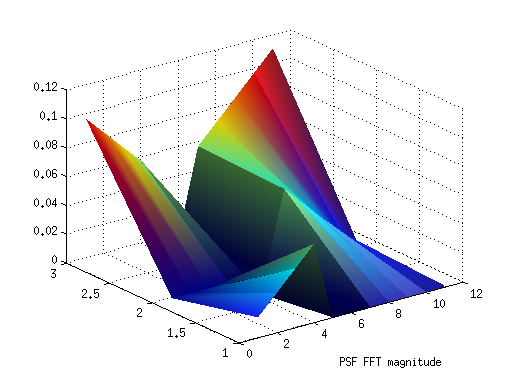
\includegraphics[scale=0.5]{../Images/psfFFT.png}
\caption{FFT of the psf}
\label{fig:psfFFT}
\end{figure}


\subsection{Lucy-Richarson}
\subsubsection{Theory behind the method}
The method was introduced in~\cite{richardson1972bayesian} and
then in~\cite{lucy1974iterative} by Richarson and Lucy respectively.
I these articles, $f$ and $g$ are considered as probability function.
\cite{richardson1972bayesian} says (translated in our notations)
``Units of enery (which may be considered as unique events)
originating at a point in $f$ are distributed at points in $g$
according to the frequencies indicated by $h$''.
However, the justification of~\cite{richardson1972bayesian} (in 1D) uses
$P(f(x)) = \frac{f(x)}{\sum_x f(x)}$ which does not seem
very appropriate.

When \cite{richardson1972bayesian} talks about energy,
that refers to the light which is quantized with photons.
That quantization gives us a reason to model the noise with
poisson distribution.
This modelization of the noise is called the shot noise and
is developped in~\cite{blanter2000shot}.
This model of the noise is used by~\cite{hebert1989generalized}.
\cite{temerinac2010tile} base on~\cite{hebert1989generalized}
and this model of the noise to show (even in 3D)
that the Lucy-Richardson algorithm gives the MLE of $f$ of this
model.

They suggest that $G \sim \pois(h * f)$ ($G$ is capitilize sinced it is a random function).
Therefore,
\begin{align*}
  L(f) & = P(g|f)\\
  & = \prod_{(x,y)} \frac{[(h*f)(x,y)]^{g(x,y)} \exp(-(h*f)(x,y))}{(g(x,y))!}\\
  l(f) & = \sum_{(x,y)} g(x,y)\log((h*f)(x,y)) - (h*f)(x,y) -\log(g(x,y)!).
\end{align*}
Let's first develop
\begin{align*}
  \fpart{(h*g)(x,y)}{f(a,b)} & = \fpart{}{f(a,b)}\sum_{(i,j)}f(i,j)h(x-i,y-j)\\
  \fpart{(h*g)(x,y)}{f(a,b)} & = h(x-a,y-b).
\end{align*}
Consequently, we have
\begin{align*}
  \fpart{l(f)}{f(a,b)} & = \sum_{(x,y)} \left(\frac{g(x,y)}{(h*f)(x,y)} - 1\right) \fpart{(h*g)(x,y)}{f(a,b)}\\
  & = \sum_{(x,y)} \left(\frac{g(x,y)}{(h*f)(x,y)} - 1\right) h(x-a,y-b)\\
  & = \left(\left(\frac{g(x,y)}{(h*f)(x,y)} - 1\right) * h(-x,-y)\right)(a,b)\\
  & = \left(\left(\frac{g(x,y)}{(h*f)(x,y)}\right) * h(-x,-y)\right)(a,b) - 1 * h(-x,-y)\\
  & = \left(\left(\frac{g(x,y)}{(h*f)(x,y)}\right) * h(-x,-y)\right)(a,b) - \left(\sum_{(i,j)} h(-x-i,-y-j)\right)(a,b).
\end{align*}
As explained in the mathematical model,
\[ \sum_{(i,j)} h(i,j) = 1 \]
so we have
\[ \nabla l(f) = \frac{g(x,y)}{(h*f)(x,y)} * h(-x,-y) - 1. \]
To get the minimum of $l(f)$, $\nabla l(f)$ needs to be 0.
Therefore % TODO Justify hessienne
\[ \frac{g(x,y)}{(h*\hat{f})(x,y)} * h(-x,-y) = 1. \]
If we multiply each side by $f(x,y)$, we get
\[ f(x,y)\left(\frac{g(x,y)}{(h*\hat{f})(x,y)} * h(-x,-y)\right) = f(x,y) \]
which can be solved iteratively using the fixed point method which gives us
\[ f_{k+1}(x,y) = f_k(x,y)\left(\frac{g(x,y)}{(h*f_k)(x,y)} * h(-x,-y)\right). \]

\section{Wiener Deconvolution}
 Another deconvolution is the wiener one. 




\section{Regularisation}
%TODO
The last deconvolution method is the deconvolution using regularized filter. 
Instead of a simple inverse 
\begin{equation}
\sum_{m,n} \left[ (g(m,n) - h(m,n)*f(m,n))^2 + \alpha (l(m,n)*f(m,n))^2 \right]
\end{equation}

\begin{equation}
\sum_{k,l} \{ [G(k,l) - H(k,l)F(k,l)]^2 + \alpha [L(k,l)F(k,l)]^2\}
\end{equation}


\begin{equation}
\hat{F}(k,l) = \frac{H(k,l)}{|H(k,l)|^2 + \alpha |L(k,l)|^2} G(k,l)
\end{equation}

\section[Compl. Treatment]{Complementary Treatment}
\begin{frame}
  \frametitle{no referential blur metric}
  
  advantage: absolute metric, no need of the original image\\
  steps:
  \begin{itemize}
  \item vertical edges (Sobel)
  \item analysing the image image by row. Everytime a pixel that is part of an edge is found, determining the local minimum and extremum on that row.
  \item local blur = distance (in pixels) between the extrema
  \item global blur = average of local blurs
  \end{itemize}
\end{frame}
